\chapter{Determining $b\bar{b}$-tagging Scale Factors for W jets in $t\bar{t}$ Events}
\label{chap:bbsf}

$t\bar{t}$ production has a large production cross section at the LHC and often makes up a substantial component of the background for physics analyses. These events have a rich final state with two b jets from each of the top decays, and hadrons or leptons from the decay of each of the Ws. Semi-leptonic events, illustrated in Figure~\ref{fig:ttbar}, are events in which one W decays to a lepton and neutrino, and the other decays hadronically. These events have a true source of missing energy (\ptmiss), and additionally can result in boosted W bosons.

Although W bosons do not decay to b-quarks (the top quark is too heavy), the $b\bar{b}$-tagger has a non-zero probability to tag one of these jets as having decayed to a $b\bar{b}$ pair. (see Section \ref{sec:baseline} for the application of $b\bar{b}$-tagging in the SUSY analysis.) This \textit{mistag} rate can, in principle, be different in simulation compared to in data. Depending on the use, it may be necessary to apply \textit{scale factors} to the simulation to correct for this difference. This appendix provides a description of how these scale factors and their uncertainties are determined.

\begin{figure}[hbp!]
\centering
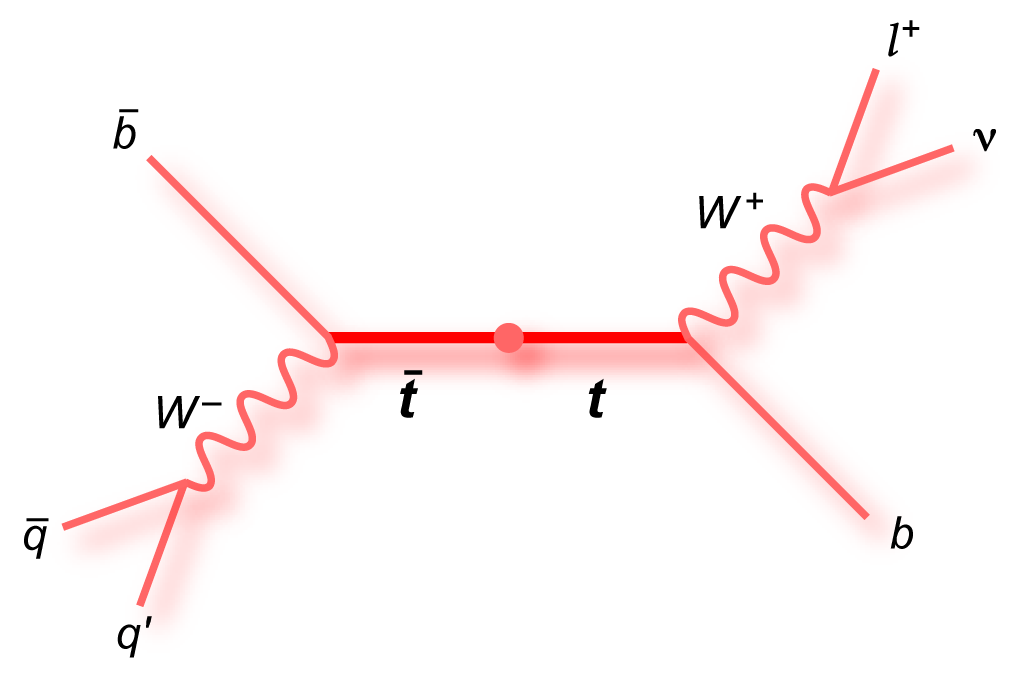
\includegraphics[width=0.4\textwidth]{figs/feynman_ttbar_ljets_beamline.png}
\caption[Diagram of a semileptonic $t\bar{b}$ event in which one W boson decays leptonically and one W boson decays hadronically.]{Diagram of a semileptonic $t\bar{b}$ event in which one W boson decays leptonically and one W boson decays hadronically \cite{ttbar}.}
\label{fig:ttbar}
\end{figure}

To obtain a clean source of hadronically decaying W bosons, events are selected that are consistent with semi-leptonic $t\bar{t}$ events. The events are obtained from a data sample with a trigger requirement of at least one muon with $p_{T}>50\,\textrm{GeV}$ and are reconstructed in the same manner as described in Chapter 6.  In particular, jets are reconstructed with the anti-kt algorithm \cite{1126-6708-2008-04-063} operated with distance parameters of 0.4 (AK4 jets) and 0.8 (AK8 jets). The events are required to have a single muon with $p_{T}>50\,\textrm{GeV}$ and $|\eta|<2.1$ and be close $(\Delta\phi < 2\pi/3)$ to a b-tagged AK4 jet, where the loose b-tagging working point of the CSV algorithm is used \cite{BTV-16-002}.  Away from this muon $(\Delta\phi > 2\pi/3)$, we require at least one AK8 jet with $p_{T}>250\,\textrm{GeV}$ and $|\eta|<2.4$, intended to be the W jet. To increase the purity of the sample, three additional criteria are applied:

\begin{itemize}

\item
The AK8 jet must be consistent with having a two-jet substructure. This requirement is made by defining a variable ``n-subjettiness'' which parametrizes the degree to which an AK8 jet is consistent with having $n$ subjets \cite{njet1, njet2}. The variable is calculated by forming a $p_{T}$ weighted sum of the $\Delta R$ distance of every particle in the jet with its nearest subjet, for some fixed number of subjets: $\tau_{N} = \frac{1}{d_{0}} \sum_{k} p_{T, k} \min \{ \Delta R_{1,k}, \Delta R_{2,k}, ..., \Delta R_{N,k} \}$, where $d_{0} = 0.8 \sum_{k} p_{T, k}$, is a normalization parameter. The ratio $\tau_{2}/\tau_{1}$ is formed to discriminate between jets with two subjets from those with one.%The bottom left of Figure~\ref{fig:dists} shows the distribution for our samples. Signal like events peak to the left.

\item
The AK8 jet mass must be between 50 and 200 GeV.  This is consistent with the W boson mass of $80.379\,\textrm{GeV}$, and tends to reject jets arising from QCD-only interactions, which tend to have lower mass.
\item
To minimize contamination from nearby objects, no AK4 jets are allowed within $\Delta R = \sqrt{(\Delta\phi)^2+(\Delta\eta)^2}<0.8$ of the selected AK8 jet.
\end{itemize}

Figure~\ref{fig:dists} (left) shows the AK8 jet mass distribution from data and simulation after all selection criteria have been applied. The distribution peaks near the W boson mass (80.379 GeV) and is dominated by the desired signal.  There is also a shoulder near the top quark mass (173.0 GeV), which arises from the merging of a W boson and a b quark into a single AK8 jet.

\begin{figure}[hbp!]
\centering
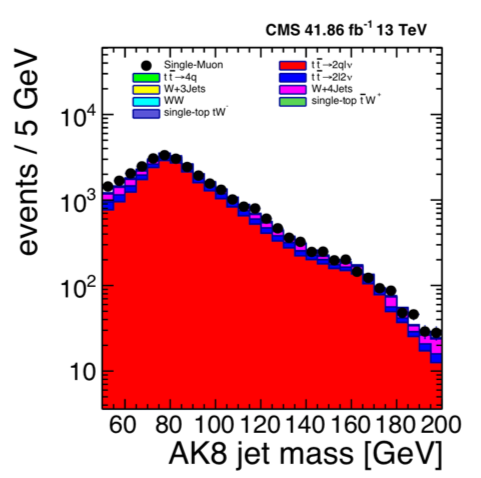
\includegraphics[width=0.465\textwidth]{figs/ak8jetmass.png}
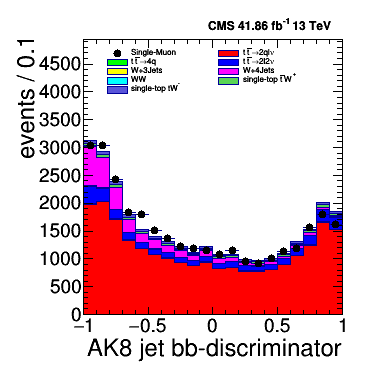
\includegraphics[width=0.48\textwidth]{figs/ak8jetbbdisc.png}
%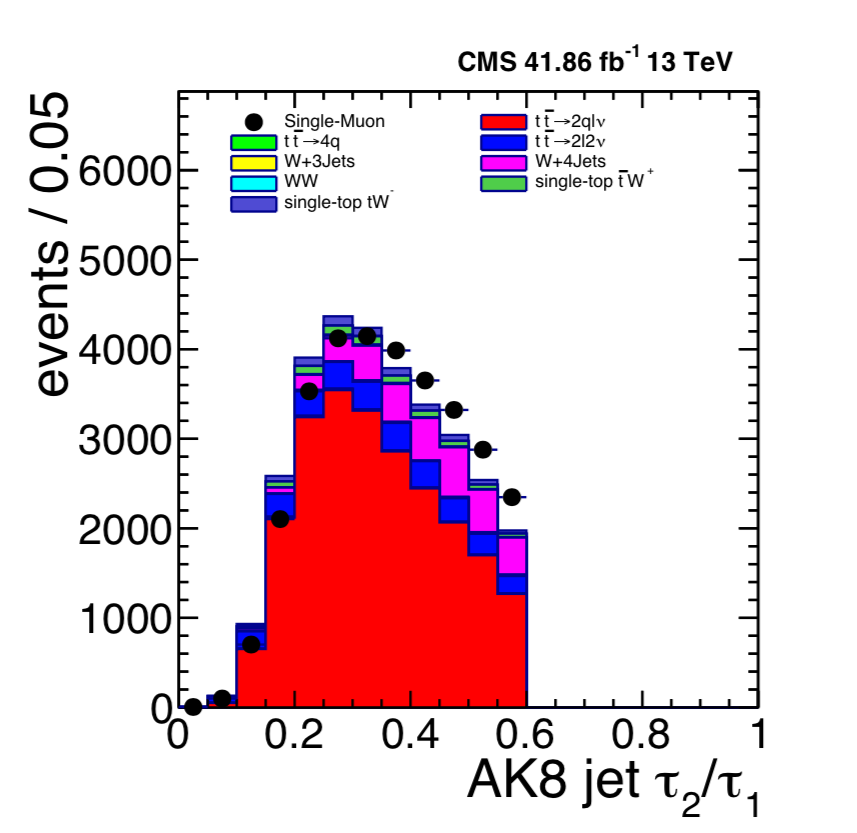
\includegraphics[width=0.465\textwidth]{figs/tau2tau1.png}
\caption[The AK8 jet mass and $b\bar{b}$-tagging discriminator distributions from data and simulation.]{The AK8 jet mass and $b\bar{b}$-tagging discriminator distributions from data and simulation. The simulation distributions are normalized by area to the data.}
\label{fig:dists}
\end{figure}

Figure~\ref{fig:dists} (right) shows the distribution of the $b\bar{b}$-tagging discriminator for data and simulation. The simulation contributions are divided into signal  and background components, where the signal contributions are inclusive $t\bar{t}$ events and the background contributions are from events with direct W boson plus jets, WW, or single-top production.  For a given working point (i.e.\ a fixed point along the x-axis), the mistag rate for the MC simulation is the ratio of the number of signal MC events above that point to the total number of signal MC events. The mistag rate for the data is calculated similarly except that the observed yields are corrected by subtracting the expected number of background events, estimated from the MC simulation:

\begin{equation}
\label{eq:mistags}
\epsilon_{mc} = \frac{ N_{b\bar{b}-tagged}^{sig, mc} } { N^{sig, mc} }, \hspace{1cm}
\epsilon_{data} = \frac{N_{b\bar{b}-tagged}^{data}-N_{b\bar{b}-tagged}^{bkg, mc}}{N^{data} - N^{bkg, mc}}, 
\end{equation}

Following this prescription, we obtain the mistag rates in data and simulation seen in Table~\ref{tab:mistag}. Four working points are defined ranging from disc$>$0.3 to disc$>$0.9. It is seen that the mistag rate in MC is higher for all working points than in data. This trend can be seen in the right-hand plot of Figure~\ref{fig:dists} - the MC under-predicts the yields with low discriminator value, and over-predicts those with a large discriminator value.

\begin{table}[hbp!]
\centering
\caption[W jet $b\bar{b}$ mistag rates in data and simulation, inclusive in $p_{T}$]{W jet $b\bar{b}$ mistag rates in data and simulation, inclusive in $p_{T}$. Statistical uncertainties only.}
\label{tab:mistag}
\begin{tabular}{c|cc}
\hline\hline
working point & data & MC\\
\hline
disc $>$ 0.3 & 0.326 $\pm$ 0.003 & 0.340 $\pm$ 0.003 \\
disc $>$ 0.6 & 0.219 $\pm$ 0.003 & 0.236 $\pm$ 0.002 \\
disc $>$ 0.8 & 0.122 $\pm$ 0.002 & 0.138 $\pm$ 0.002 \\
disc $>$ 0.9 & 0.058 $\pm$ 0.001 & 0.067 $\pm$ 0.001 \\
\hline\hline
\end{tabular}
\end{table}

The scale factors are then formed by taking the ratio of the mistag rate in data to that of simulation:
\begin{equation}
\label{eq:sf}
\textrm{scale factor} = \frac{\epsilon_{data}} {\epsilon_{mc}}
\end{equation}

Table~\ref{tab:sf} shows the scale factors, binned in jet $p_{T}$, for the four different working points. The uncertainties are the result of summing in quadrature the statistical and two additional systematic uncertainties: The first systematic uncertainty originates from subtracting the background from the data using the MC. The uncertainty in the cross section of the background contributions is estimated to be 30\%, which results in uncertainties of 2, 4, and 6\% for the low, medium, and high $p_{T}$ bins, respectively.  The second systematic uncertainty arises from a known difference in the $p_{T}$ spectra of top quarks between data and simulation \cite{ttbar}. We assess the systematic uncertainty by comparing results when the top quark $p_{T}$ spectra is and is not reweighted to match the data.  This results in 0, 1, and 2\% uncertainties for the low, medium, and high $p_{T}$ bins, respectively.

\begin{table}[hbp!]
\centering
\caption{Summary of scale factors for $b\bar{b}$-tagging W jets in $t\bar{t}$ events.}
\label{tab:sf}
\begin{tabular}{c|ccc}
\hline\hline
working point & $250 < p_{T} < 350\,\textrm{GeV}$ & $350 < p_{T} < 430\,\textrm{GeV}$ & $p_{T}>430\,\textrm{GeV}$\\
\hline
disc $>$ 0.3 & 0.939$\pm$0.026 & 1.007$\pm$0.055 & 0.996$\pm$0.079 \\
disc $>$ 0.6 & 0.922$\pm$0.027 & 0.967$\pm$0.057 & 0.902$\pm$0.082  \\
disc $>$ 0.8 & 0.875$\pm$0.030 & 0.939$\pm$0.063 & 0.893$\pm$0.090  \\
disc $>$ 0.9 & 0.855$\pm$0.036 & \multicolumn{2}{c}{0.914$\pm$0.068} \\
\hline\hline
\end{tabular}
\end{table}
